\section{Mapping Node}

As can be seen in figure \ref{ImplOverview} the mapping node has a central position in the system. It is also the largest node in terms written code. This section is split into two parts, the class structure and the execution. 

\subsection{Class Stucture}

In figure \ref{mapping overview} the general structure of the mapping node is show. The \texttt{TopologicalMapper} class is the main class in this structure, holding an instance of the  \texttt{RoomMapper} class for every room. The \texttt{RoomMapper} class is derived from the \texttt{SlamGmapper} class, which does the 2D SLAM using Gmapping. Instead of putting the other types of maps into the particles, which would have resulted in making major changes to Gmapping, the \texttt{RoomMapper} class holds a separate mapping class for every type of map and every particle. 

\begin{figure}
  \centering
  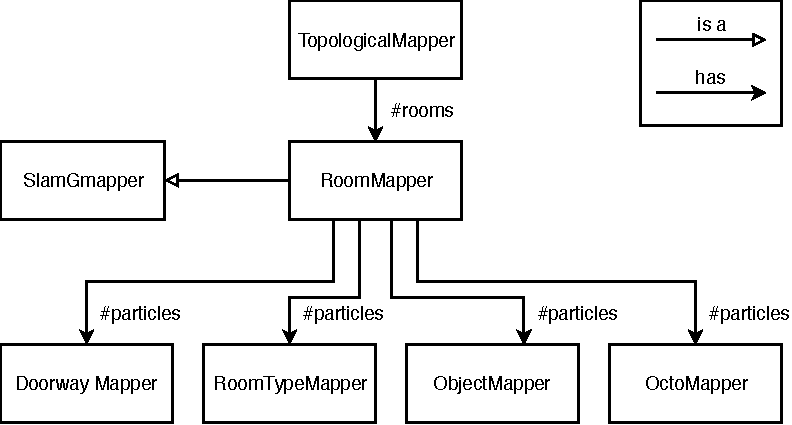
\includegraphics[width=0.9\textwidth,clip]{figures/MappingClassDiagram.pdf}
  \caption[Mapping node structure]{An overview over structure of the mapping node}
  \label{mapping overview}
\end{figure}

In listing \ref{TopologicalMapper} the most important member variables and methods of the \texttt{TopologicalMapper} class are shown. 

\begin{minipage}{\linewidth}
\begin{lstlisting}[language=Python, caption=\texttt{TopologicalMapper} class,frame=single, label=TopologicalMapper]
   //members
   RoomMapper[] room_mapper
   int current_mapper
   bool[] room_explored
   topologicalMapServiceResponse topology
   bool[] room_changed
   int current_action
   
   //methods
   run()
   
   pointcloudCallback(point_cloud)
   laserCallback(laser_scan)
   doorwayCallback(doorway_detections)
   visionCallback(vision_result)
   currentActionCallback(current_action)
   exploredCallback(explored)
   
   topologicalMapServiceCallback()
   objectMapServiceCallback(room_id, object_id)
   
\end{lstlisting}
\end{minipage} 

Beside an array of \texttt{RoomMapper} it also has variables to keep track of the current room and which rooms are explored. The latter is important in the generation of the high-level attributes during the \texttt{topologicalMapSrv} service. The variable topology stores the result of the last \texttt{topologicalMapSrv} service execution and \texttt{room{\_}changed} keeps track of which rooms' maps were updated since the last execution of the \texttt{topologicalMapSrv} service. Together they are used to avoid unnecessary calculations on unchanged room maps. Also the current action is stored to decide if the doorways have to be blocked by virtual obstacles.

The \texttt{TopologicalMapper} class contains the \texttt{run()} function, which is started during initialization and returns when the node is terminated. It also has the callback functions for all messages and services.

The code in the ROS-node for Gmapping was the starting point for the implementation of the \texttt{SlamGmapper} class, whose most important member variables and methods are shown in listing \ref{SlamGmapper}.

\begin{minipage}{\linewidth}
\begin{lstlisting}[language=Python, caption=\texttt{SlamGmapper} class,frame=single, label=SlamGmapper]
   //members
   ParticleFilter[] particle_filter 
   OccupancyGrid map
   Transform map_to_odometry_transform
   
   //methods
   processLaser(laser_scan)
   
\end{lstlisting}
\end{minipage}

This class is the interface to the Gmapping library used for 2D SLAM. The \texttt{ParticleFilter} class it holds is derived from Gmapping's particle filter class and has additional functionality for map switching and access to the particles. It has variables containing the currently most likely map and the transformation between the map and the odometry coordinate frames. While the transformation is only updated when a laser scan is processed the robot pose can still change based on the odometry data. The \texttt{processLaser()} is called to update the localization and the map.

The \texttt{RoomMapper} class is the main class for the mapping within a room and an overview over the most important members and methods is given in listing \ref{RoomMapper}. 

\begin{minipage}{\linewidth}
\begin{lstlisting}[language=Python, caption=\texttt{RoomMapper} class,frame=single, label=RoomMapper]
   //members
   OctoMapper[] octo_mapper
   ObjectMapper[] object_mapper
   RoomTypeMapper[] roomtype_mapper
   DoorwayMapper[] doorway_mapper
   
   //methods
   activate(robot_pose)
   deactivate()
   
   processCloud(point_cloud)
   processDoorway(doorway_detections)
   processVision(vision_result)
   
\end{lstlisting}
\end{minipage} 

It inherits the 2D SLAM functionality from the \texttt{SlamGmapper} class and also holds the mappers for all the other information. It can be activated and deactivate and has functions to update the different map types.

The \texttt{OctoMapper} class is based on the code of the octomap{\_}server ROS-node. It is the interface to the OctoMap library. In addition to the  \texttt{processCloud()} function, which is called to update the 3D map, it has the \texttt{projectDown()} function used project the obstacles in the 3D map into the 2D map.

\begin{minipage}{\linewidth}
\begin{lstlisting}[language=Python, caption=\texttt{OctoMappe} class,frame=single, label=OctoMapper]
   //members
   Octree octree
      
   //methods   
   processCloud(point_cloud)  
   projectDown(map2D)
   
\end{lstlisting}
\end{minipage} 

The \texttt{RoomTypeMapper} class contains 60 instances of the \texttt{RoomTypeMap} class, one for each room type. In listing \ref{RoomTypeMapper} the most important member variables and methods of the \texttt{RoomTypeMapper} class and the \texttt{RoomTypeMap} class are shown. 

\begin{minipage}{\linewidth}
\begin{lstlisting}[language=Python, caption=\texttt{RoomTypeMapper} class,frame=single, label=RoomTypeMapper]
   //members
   RoomTypeMap[] room_type_maps
      cv::Mat probability_map
      cv::Mat seen_count_map
      float resolution
      cv::Point origin
   
   //methods
   updateMaps(vision_result, particle_pose)
   
\end{lstlisting}
\end{minipage} 

The \texttt{RoomTypeMap} class is implemented using OpenCV's \texttt{cv::Mat} to represent the two dimensional grid. The \texttt{probability{\_}map} contains the probabilities of the given room type for all cells in the map. The \texttt{seen{\_}count{\_}map} is used to determine which cells were seen. This information is important when estimating the object probability in unseen areas. In addition the resolution and the origin are stored, so transforming world coordinates to map coordinates and vice verse is possible. The \texttt{updateMaps()} function is called to update the map.


The \texttt{ObjectMapper} class contains 61 instances of the \texttt{ObjectMap} class, one for each object type. In listing \ref{ObjectMapper} the most important member variables and methods of the \texttt{ObjectMapper} class and the \texttt{ObjectMap} class are shown. 

\begin{minipage}{\linewidth}
\begin{lstlisting}[language=Python, caption=\texttt{ObjectMapper} class,frame=single, label=ObjectMapper]
   //members
   ObjectMap object_maps
      cv::Mat[] probability_map
      cv::Mat[] seen_count_map  
      float resolution
      cv::Point origin
      
      updateMap(vision_result)
      
   //methods
   updateMaps(vision_result, particle_pose)
   
\end{lstlisting}
\end{minipage} 

The \texttt{ObjectMap} class is implemented using an array of OpenCV's \texttt{cv::Mat}. Each \texttt{cv::Mat} is a slice of the 3D map grid map. The \texttt{probability{\_}map}, the \texttt{seen{\_}count{\_}map}, the resolution and the origin are similar to those in the \texttt{RoomTypeMap} class. The \texttt{updateMaps()} function is called to update the maps. The \texttt{ObjectMap} class also has its own \texttt{updateMap()} function because every object type can be updated independently.

The \texttt{DoorwayMapper} class holds an array containing all doorways found in this room. The \texttt{pose{\_}array} member stores the last poses for the running average filter. Beside the pose of the doorway the \texttt{Doorway} class contains information about its corresponding doorway in the other room. This design is easy to maintain, though the access to the topological structure is more complicated. However, the topological structure is not needed frequently, only on map switches and \texttt{topologicalMapSrv} service requests. The \texttt{processDoorway()} function is called to update the doorway poses or insert a new doorway.

\begin{minipage}{\linewidth}
\begin{lstlisting}[language=Python, caption=\texttt{DoorwayMapper} class,frame=single, label=DoorwayMapper]
   //members
   Doorway[] doorways
      Pose pose
      Pose[] pose_array
      int id
      int counterpart_id
      int this_room
      int other_room
   
   //methods
   processDoorway(doorway_detections)
   
\end{lstlisting}
\end{minipage} 


\subsection{Execution}

This node is implemented using multiple threads to distribute the computational load and to avoid that computational expensive tasks block the rest of the execution. 

After the initialization the main thread calls the \texttt{run} function of the \texttt{TopologicalMapper}, which executes the main processing loop. The main processing loop is shown in figure \ref{mainLoop}.

\begin{figure}[h]
  \centering
  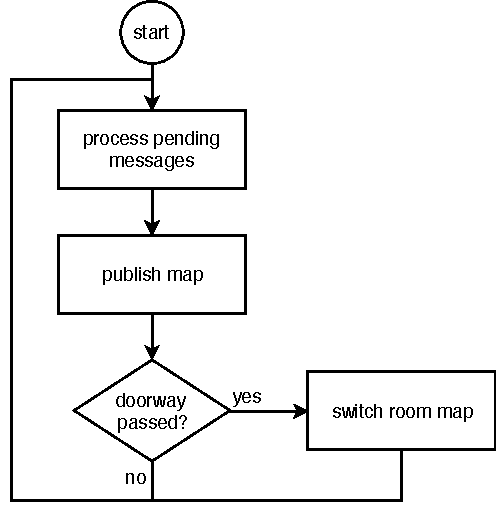
\includegraphics[width=0.5\textwidth]{figures/mainLoop.pdf}
  \caption[Main processing loop]{The main processing loop of the mapping node} 
  \label{mainLoop}
\end{figure}

First the correct callbacks for all pending messages are executed. Most of the code gets called this way. After all messages are processed the 2D map for navigation is created and published. The last step in the loop is to check if a doorway was passed and, if necessary, execute the room map switch.

\subsubsection{Message processing}

Six types of message can be received, all received in the \texttt{TopologicalMapper}. The current{\_}high{\_}level{\_}task messages and the exploration{\_}finished messages are processed directly in the \texttt{TopologicalMapper} to update the corresponding variables. The other messages are forwarded to the \texttt{RoomMapper} of the current room. 

The processing of the \texttt{laser{\_}scan{\_}filtered} message involves calling the \texttt{processLaser} function of the \texttt{RoomMapper} of the current room, which sends the laser scan to Gmapping for localization and mapping. Resampling of the particles, which involves replacing particles with copies of existing ones, can happen there. The same replacing has to be done for all mappers of the \texttt{RoomMapper}, so particles and mappers fit together after resampling. The extended ParticleFilter class allows access to the result of the resampling, which allows to do the correct replacement of the mappers after the laser scan was processed. The transformation between the map coordinate frame of the best particle and the odometry frame is done in a separate thread to ensure regular publishing.

The 3D mapping is done in a separate thread because the 3D mapping takes relatively much time. This way the computational load is distributed and the other mapping is not slowed down. Therfore the \texttt{processCloud} function of the \texttt{RoomMapper} of the current room only stores \texttt{main{\_}camera/pointcloud} message in a buffer. The thread for 3D mapping idles until a new message is in the buffer and executes the map update. First all operations independent of the particle are executed. These are the transformation of the point cloud from the camera coordinate frame into the robot coordinate frame and the split into two point clouds, one for points near the ground and one for points at heights considered in the 3D map. These are then transformed into the map coordinate frames of the particles and the \texttt{processCloud} function of the corresponding \texttt{OctoMapper} is called. Using the point clouds and ray-tracing a list of cells containing points and a list of visible cells containing no points are created, where the point cloud with points near the ground is only used for the latter. This way no 3D mapping is done for points near the ground. Then the 3D map is updated using the two lists. The ray-tracing and the map update is done using the OctoMap library. 

For good results the transformation from the robot coordinate frame into the coordinate frame of the particles has to be accurate, especially the rotation. Particle poses are only known at times a processed laser scan was recorded, but for accurate mapping the particle pose at the time the point cloud was recorded is necessary. Therefore the particle pose at that time is estimated using the available particle pose nearest in time and the odometry data to estimate the movement of the robot in between. 

In the callback for the \texttt{vision{\_}result} message the \texttt{processVision} function of the \texttt{RoomMapper} of the current room is called. For every particle the particle pose is calculated as described above and the \texttt{updateMaps} functions of the corresponding \texttt{RoomTypeMapper} and the corresponding \texttt{ObjectMapper} are called, where in the latter the \texttt{updateMap} for all object types is called. There the map update is done according to section \ref{Room-Type-Map} and section \ref{Object-Map}.

The doorway poses in the \texttt{door{\_}detections} message are transformed into the map frames of all particles and the \texttt{processDoorway} functions of the corresponding \texttt{DoorwayMapper} instances are called. According to section \ref{Doorway Mapping} the decision is made if it is a new doorway or another detection of an already found doorway. If it is a new doorway a new instance of \texttt{Doorway} is added to the array of doorways. All elements in the \texttt{pose{\_}array} and \texttt{pose} are set to the pose of the detected door, a new id is generated for the doorway and the values of \texttt{counterpart{\_}id} and \texttt{other{\_}room} are set to -1. -1 signals that the doorway was never passed. If the detection is from an already found doorway, the oldest element in the \texttt{pose{\_}array} is replaced by the pose of the doorway detection and the average in the \texttt{pose{\_}array} is assigned to the \texttt{pose} variable. To calculate the average orientation the corresponding point on the unit circle is calculated for all orientations of the poses in the \texttt{pose{\_}array}. The angle of the average of these points is the average orientation.

The creation of the map used for navigation and low-level planning in regular intervals is done as described in section \ref{topomapping}. Additionally, if \texttt{current{\_}action} is not move through doorway, the doorways have to be blocked. This is done by setting cells on a line short line perpendicular to the doorway poses to occupied. This created map is then published. 




\subsection{Implementation Details}






















\subsection{Processing of Messages}

All messages are fetched by the \texttt{TopologicalMapper} class and forwarded to the \texttt{RoomMapper} instance of the current room. The \texttt{TopologicalMapper} class has a different callback function for all the different messages and also in this section the processing of the messages is described separately.

\subsubsection{Laser scan}

The laser scan messages are forwarded to the \texttt{processLaser()} function of the \texttt{SlamGmapper} class. The \texttt{processLaser()} function is basically the same as in the ROS node for Gmapping, with one exception. For the particle filter to work resampling is needed. During the resampling unlikely particles are replaced by copies of more likely particles. This has also to be done with the mappers of the other maps. To get the information about the resampling a own particle filter class is derived from the Gmapping particle filter class, which stores if resampling was done and how the particles were changed. Using this information the replacement of the other mappers is done after the processing of the laser scan.

\subsubsection{Point cloud}

The point cloud messages are forwarded to the \texttt{processCloud()} function of the \texttt{RoomMapper} class. This function copies the point cloud into a buffer to be processed by the thread for 3D mapping. This runs in a loop and checks, if a new point cloud is in the buffer. If this is the case the operations independent of the particle are done. Those are the transformation from the camera coordinate frame into the robot coordinate frame and the segmentation of the point cloud into ground points and points in the mapped height range. This segmentation is done because the ground should not be mapped. 

The remaining steps are executed for every particle individually. First the poses of the particles at the time the point cloud was recorded are calculated. The pose of a particle exists only for the times, when a processed laser scan was recorded. However, especially the orientation of the particle has to be accurate because even small deviations in the orientation causes points at the maximum range of the camera to be far off. Therefore the particle pose is interpolated using the data of the odometry. Using the particle pose the two parts of the point cloud are transformed into the map coordinate frame of the particle. 

These transformed point clouds are the sent to the corresponding \texttt{OctoMapper}. The code for the map update is basically the same as in the octomap{\_}server ROS-node. 

\subsubsection{Vision result}

The \texttt{VisionResult} message contains both the results of the room type classification and the object detection. So for every particle two maps are updated. 

First the update of the Room-Type-Map is done. To do this the \texttt{updateMaps()} functions of the  \texttt{RoomTypeMapper} of all the particles of the current \texttt{RoomMapper} are called with \texttt{VisionResult} message and the pose of the corresponding particle as parameters. The pose of the particle is calculated as described in the processing of the point cloud. 

The update of the probabilities is done according to \ref{Room-Type-Map}. When a cell is updated the the corresponding value in the \texttt{seen{\_}count{\_}map} is incremented. When the area to update goes beyond the map a fixed number of columns or rows is added to the map, so the updated region fits into the map. 

For the update of the Object-Map the detection samples are transformed into the map coordinate frames of the particles. The update of the object probabilities is done according to \ref{Object-Map} and the map resize is done the same way as in the \texttt{RoomTypeMapper}.

\subsubsection{Doorway detection}

If the doorway detection message contains at least one doorway the call to the \texttt{DoorwayMapper}s is done similar to for the other messages. 

\subsection{Main Execution Loop}

In this node four threads are running simultaneously. One thread is just for publishing the transformation between map coordinate frame and odometry coordinate frame, which is an indirect way of publishing the robot pose. A second thread is used for processing the service requests. For every room a worker thread exists for 3D mapping, but only the thread of the current room is running. This leaves the main thread, whose execution is now described in more detail. Beside the receiving, forwarding to the current room mapper and processing of the message, which will be described in the next section, it has two additional tasks. 

The first is the creation and publishing of the map used for navigation and low-level planning in regular intervals. The creation involves two steps. The first one is inserting the obstacles found with 3D mapping. Listing \ref{Downprojection} shows how this is done. A second thread is working on the 3D map, so getting exclusive access to the 3D map is essential. The \texttt{getProjection()} function calculates the projection of the node into the 2D grid map. The cells in this projection are then set occupied.

\begin{minipage}{\linewidth}
\begin{lstlisting}[language=Python, caption=Inserting obstacles found in 3D map,frame=single, label=Downprojection]
   navigation_map = room_mapper[current_room].get2DMap()
   lock3DMap()
   for node in room_mapper[current_room].
                  octo_mapper[best_particle].octree.nodes:
      if node.getOccupancy() > threshold:
         navigation_map.setOccupied(node.getProjection())
   unlock3DMap()
   publishNavigationMap()
\end{lstlisting}
\end{minipage} 

The second task is detecting if a doorway is passed and if this is the case executing the map switch. The detection of a doorway passing is shown in listing \ref{doorway passing}. 

\begin{minipage}{\linewidth}
\begin{lstlisting}[language=Python, caption=Detection of doorway passing,frame=single, label=doorway passing]
   for doorway in room_mapper[current_room].
                     doorway_mapper[best_particle].doorways:
      pose = doorway.pose.inverse()*robot_pose
      if pose.x > threshold1 and pose.y < threshold2:
         return doorway
   return Doorway()
\end{lstlisting}
\end{minipage} 

If a doorway was passed the map switch is executed. There are two cases, the other room was visited before or not. In both cases the \texttt{deactivate()} function of \texttt{room{\_}mapper[current{\_}room]} is executed, which reduces the number of particles to one by discarding all particles except the best particle and all mappers except those of the best particle. If the other room was never visited, which is the case if the \texttt{other{\_}room} variable of the passed doorway is negative, 

There the number of particles in the particle filter is reduced to one, leaving only the best particle. Gmapping provides a function for this. Using the index of the best particle stored before all other instances of the mappers are removed from the mapper arrays. If the other room was already visited, the transformation between the passed doorway and the counterpart of the doorway in the other room  is calculated. 

\subsection{Processing of Service Requests}

The two services the mapping node advertises are the \texttt{ObjectProbabilityMapSrv} service and the \texttt{TopologicalMapSrv} service. A lot of code is shared in 

\begin{lstlisting}[language=Python, caption=mapping/TopologicalMapSrv,frame=single, label=TopologicalMapService]
   RoomMsg[] rooms
      int16 id
      float32 obj_prob
      int16[] doorways # doorways in the room
      float32[] to_doorway_times
      float32 search_time
      float32 expected_search_time
   int16 curr_room
   DoorwayMsg[] doorways
      int16 room1
      int16 room2
      geometry_msgs/Pose door1_pose # doorway pose in room 1
      geometry_msgs/Pose door2_pose # doorway pose in room 2
      float32[] dists # distances to other doorways
\end{lstlisting}

\begin{lstlisting}[language=Python, caption=mapping/ObjectProbabilityMapSrv,frame=single,    label=ObjectProbabilityMapService]
   int16 room_id
   int16 id
   ---
   ObjectMapMsg map
      int16 width
      int16 height
      int16 z_steps
      int16 origin_x # position of the origin in the map
      int16 origin_y
      float32 resolution
      float32[] data
\end{lstlisting}